\documentclass[tikz,border=12pt]{standalone}
\usepackage{amsmath,amssymb}
\usetikzlibrary{arrows.meta,angles,quotes,calc,decorations.pathreplacing}

\begin{document}
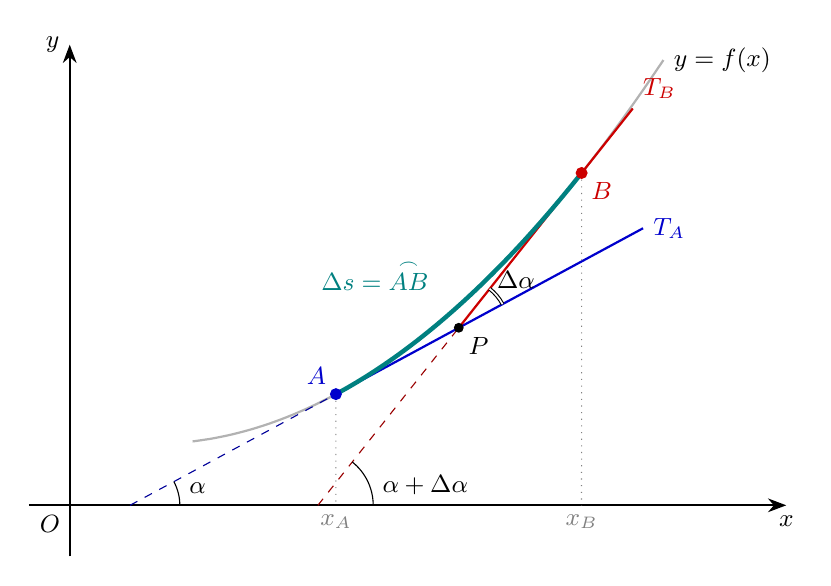
\begin{tikzpicture}[>=Stealth, scale=1.3, font=\small]

    % --- 坐标轴 ---
    % 将 y 轴左移至 x = -0.8，避免与切线虚线相交
    \draw[->, thick] (-1.2, 0) -- (6.2, 0) node[below] {$x$};
    \draw[->, thick] (-0.8, -0.5) -- (-0.8, 4.5) node[left] {$y$};
    \node[below left] at (-0.8, 0) {$O$};

    % --- 曲线 y = 0.15*x^2 + 0.6 ---
    \draw[thick, gray!60, domain=0.4:5.0, smooth, variable=\x] 
        plot ({\x}, {0.15*\x*\x + 0.6}) node[right, text=black] {$y = f(x)$};

    % --- 关键几何坐标计算 ---
    % A(1.8, 1.086), 切线斜率 k1 = 0.54, 倾角 alpha = 28.37°
    % B(4.2, 3.246), 切线斜率 k2 = 1.26, 倾角 alpha + Delta alpha = 51.56°
    % 切线A与x轴交点 XA = (-0.211, 0)
    % 切线B与x轴交点 XB = (1.624, 0)
    % 两切线交点 P = (3.0, 1.734)
    \coordinate (XA) at (-0.211, 0);
    \coordinate (XB) at (1.624, 0);
    \coordinate (A)  at (1.8, 1.086);
    \coordinate (B)  at (4.2, 3.246);
    \coordinate (P)  at (3.0, 1.734);
    
    % 切线端点延伸
    \coordinate (TA_ext) at (4.8, 2.706);
    \coordinate (TB_ext) at (4.7, 3.876);
    
    % 辅助水平参考点
    \coordinate (XA_h) at (1.2, 0);
    \coordinate (XB_h) at (3.0, 0);

    % --- 切线 ---
    % 切线 1 (过 A)
    \draw[dashed, blue!60!black] (XA) -- (A);
    \draw[thick, blue!80!black] (A) -- (TA_ext) node[right, text=blue!80!black] {$T_A$};
    
    % 切线 2 (过 B)
    \draw[dashed, red!60!black] (XB) -- (P);
    \draw[thick, red!80!black] (P) -- (TB_ext) node[above right, text=red!80!black] {$T_B$};

    % --- 突出显示的弧段 Delta s ---
    \draw[ultra thick, teal, domain=1.8:4.2, smooth, variable=\x] 
        plot ({\x}, {0.15*\x*\x + 0.6});
    \node[teal, above left] at (2.8, 2.0) {$\Delta s = \overset{\frown}{AB}$};

    % --- 垂线辅助线 ---
    \draw[dotted, gray] (A) -- (1.8, 0) node[below] {$x_A$};
    \draw[dotted, gray] (B) -- (4.2, 0) node[below] {$x_B$};

    % --- 角度标注 ---
    % 角 alpha (切线 A 与 x 轴夹角)
    \pic[draw, "$\alpha$", angle radius=18pt, angle eccentricity=1.4] 
        {angle = XA_h--XA--A};

    % 角 alpha + Delta alpha (切线 B 与 x 轴夹角)
    \pic[draw, "$\alpha + \Delta\alpha$"{xshift=28pt, yshift=2pt}, angle radius=20pt] 
        {angle = XB_h--XB--B};

    % 外角 Delta alpha (两切线交点 P 处的夹角)
    \pic[draw, double, "$\Delta\alpha$", angle radius=18pt, angle eccentricity=1.5] 
        {angle = TA_ext--P--TB_ext};

    % --- 标注关键点 (A 设为蓝色，B 设为红色) ---
    \filldraw[blue!80!black] (A) circle (1.5pt) node[above left, text=blue!80!black] {$A$};
    \filldraw[red!80!black]  (B) circle (1.5pt) node[below right, text=red!80!black] {$B$};
    \filldraw[black]         (P) circle (1.2pt) node[below right] {$P$};

\end{tikzpicture}
\end{document}